\documentclass{amsart}
\usepackage[utf8]{inputenc}

\usepackage{fullpage}
\usepackage{bm}
\usepackage{bbm}
\usepackage{physics}
\usepackage{graphicx}
\usepackage{subcaption}
\usepackage{natbib}
\usepackage[colorlinks]{hyperref}
\usepackage{xifthen}

\DeclareMathOperator*{\Argmax}{argmax}
\DeclareMathOperator*{\Argmin}{argmin}
\DeclareMathOperator*{\KLOp}{KL}
\DeclareMathOperator*{\PrOp}{\mathbb{P}}
\DeclareMathOperator*{\EvOp}{\mathbb{E}}
\DeclareMathOperator*{\VarOp}{\mathbb{V}ar}

\newcommand{\CD}{\mathcal{D}}
\newcommand{\CH}{\mathcal{H}}
\newcommand{\CX}{\mathcal{X}}
\newcommand{\CY}{\mathcal{Y}}

\newcommand{\RR}{\mathbb{R}}
\newcommand{\NN}{\mathbb{N}}

\newcommand{\UnifDist}{\text{Unif}}
\newcommand{\NormalDist}{\mathcal{N}}
\newcommand{\BetaDist}{\text{Beta}}

\renewcommand{\Vec}[1]{\bm{#1}}
\newcommand{\Mat}[1]{\mathbf{#1}}

\newcommand{\KL}[2]{\KLOp(#1\parallel#2)}
\newcommand{\Abs}[2][]{%
  \left\lvert#2\right\rvert\ifthenelse{\isempty{#1}}{}{_{#1}}%
}
\newcommand{\Norm}[2][]{%
  \left\lVert#2\right\rVert\ifthenelse{\isempty{#1}}{}{_{#1}}
}
\renewcommand{\Pr}[2][]{%
  \PrOp\ifthenelse{\isempty{#1}}{}{_{#1}}\left[#2\right]
}
\newcommand{\Ev}[2][]{%
  \EvOp\ifthenelse{\isempty{#1}}{}{_{#1}}\left[#2\right]
}
\newcommand{\Var}[2][]{%
  \VarOp\ifthenelse{\isempty{#1}}{}{_{#1}}\left[#2\right]
}

\newtheorem{theorem}{Theorem}
\newtheorem{proposition}[theorem]{Proposition}
\newtheorem{lemma}[theorem]{Lemma}
\newtheorem{corollary}[theorem]{Corollary}
\theoremstyle{definition}
\newtheorem{remark}[theorem]{Remark}
\newtheorem{definition}[theorem]{Definition}
\newtheorem{problem}[theorem]{Problem}
\newtheorem{example}[theorem]{Example}

\title{
  Math 651: Course Project Report\\
  Bridging PAC-Bayes Theory and Bayesian Inference
}
\author{
  Saibal De
}

\begin{document}

\maketitle

\section{Introduction}

In the classical approach to science and engineering problems, we develop models
from first-principles, such as Newton's laws of mechanics and Maxwell's theory
of electromagnetism. We then test the predictions of these models with
experimental data. But in many cases, the first principles are unknown, and the
data is readily available ---this has led to a paradigm shift, where we aim to
discover the first principles from the data.

In such an approach, there are two primary stages: we first construct an
appropriate model using the data, then test the model by making predictions on
unseen data. The first stage falls inside the regime of estimation---many
frameworks have been developed over the last centuries for this purpose. One of
the most popular of such frameworks is Bayesian inference, which provides a
systematic rule for updating beliefs, e.g.\ model parameters, based on evidence,
i.e.\ data (see \citet{bishop2006pattern} and
\citet{ghahramani2015probabilistic} for more details). However, the second stage
of our data-driven learning approach, commonly referred to as generalization,
poses a challenge.

\subsection{Quick Review of PAC Learning}

Following the pioneering work of \citet{vapnik1971uniform}, which provides
uniform bounds on generalization error, the probably approximately correct (PAC)
learning framework has been developed to address this question (see
\citet{shalev2014understanding} for an excellent survey of this topic). In the
context of supervised learning, this problem is posed as follows: let $\CX$
denote the feature space of data, and $\CY$ the label space. We have i.i.d.\
samples $S = \{(x_1, y_1), \ldots, (x_n, y_n)\}$ generated from a data
distribution $\CD$ defined over $\CX \times \CY$. Our goal is to learn a
function $f : \CX \to \CY$ that would, first, fit the available training data
(the estimation stage), and then will predict the label $y = f(x)$ given any
feature $x \in \CX$ ``correctly''. In a typical scenario, we would choose a
candidate $h$ from some hypothesis class $\CH$ consisting of functions from the
feature space to the label space. We also have a loss function $L : \CH \times
\CX \times \CY \to \RR$ that describes the closeness of of a predicted label
$h(x)$ given a feature $x$ and hypothesis $h$, and its true label $y$. In
theory, we would want to return a hypothesis $h^*$ that minimizes the true risk
(a.k.a.\ generalization error)
\begin{equation}
  R_\CD^L(h) := \Ev[(x, y) \sim \CD]{L(h, x, y)}
\end{equation}
However, we cannot compute this quantity as $\CD$ is unknown. Hence we take the
advantage of the i.i.d.\ sampling assumption and come up with the empirical risk
(a.k.a.\ training error)
\begin{equation}
  \hat{R}_S^L(h) := \frac{1}{n} \sum_{i = 1}^n L(h, x_i, y_i)
\end{equation}
From the law of large numbers, we know that as the sample size $n$ approaches
infinity, the empirical risk approaches the true risk by the law of large
numbers. Therefore, we intuitively expect the hypothesis constructed using the
training error to be the ``more correct'' as the number of samples increase. The
PAC theory provides theoretical guarantees for this in terms of VC dimension (a
measure of complexity) of hypothesis classes:

\begin{definition}[Shattering for Indicator Functions]
  A set of indicator functions $\CH$, with $h : \CX \to \{0, 1\}$ for each $h
  \in \CH$, is said to shatter a set of points $x_1, \ldots, x_n \in \CX$ if any
  two such points can be distinguished by at least one element $h \in \CH$, or
  equivalently, if the set $\{(h(x_1), \ldots, h(x_n)) : h \in \CH\}$ has
  cardinality $2^n$.
\end{definition}

\begin{definition}[VC Dimension for Indicator Function Classes]
  The VC dimension of a set $\CH$ of indicator functions is the maximum number
  of arbitrary points it can chatter.
\end{definition}

\begin{definition}[VC Dimension for Real Valued Function Classes]
  Let $\CH$ be a class of functions of the form $h : \CX \to \CY \subseteq \RR$.
  For any $y \in \CY$, define the indicator function class $\CH_y = \{h_y : h
  \in \CH\}$ where
  \begin{equation}
    h_y(x) = \mathbbm{1}_{h(x) \geq y}
  \end{equation}
  Then the VC dimension of $\CH$ is defined as $\sup_{y \in \CY}
  \text{VCdim}(\CH_y)$.
\end{definition}

We now state the following results from \citet[Sections 4.3.1 and
4.3.2]{cherkassky2007learning}:

\begin{theorem}[Generlization Error Bounds]
  Suppose $\CH$ is a hypothesis class with VC dimension $d$ and let $n$ be the
  number of i.i.d.\ training samples. Then for any bounded non-negative loss
  function $L$ (e.g.\ the 0-1 loss for classification) we have
  \begin{equation}
    \label{eq:generalization-classification}
    R_\CD^L(h) \leq \hat{R}_S^L(h) + \frac{\epsilon}{2} \qty[1 + \sqrt{1 +
    \frac{4}{\epsilon} \hat{R}_S^L(h)}] \quad \text{with probability at least }
    1 - \delta \text{ over } S \sim \CD^n
  \end{equation}
  and for any non-negative loss function $L$ (e.g.\ the squared loss for
  regression) we have
  \begin{equation}
    \label{eq:generalization-regression}
    R_\CD^L(h) \leq \frac{\hat{R}_S^L(h)}{(1 - c \sqrt{\epsilon})_+} \quad
    \text{with probability at least } 1 - \delta \text{ over } S \sim \CD^n
  \end{equation}
  where $x_+ = \max\{x, 0\}$ and
  \begin{equation}
    \epsilon = a_1 \frac{d [\log (a_2 n / d) + 1] - \log (\delta / 4)}{n}
  \end{equation}
  and $0 < a_1 \leq 4$, $0 < a_2 \leq 2$. These bounds hold simultaneously for
  all $h \in \CH$.
\end{theorem}

\subsection{Limitations of PAC Learning}

We note that these bounds are useless when the VC dimension $d$ is infinite.
This suggests a close connection between learnability and VC dimension of a
hypothesis class \citep[Sections 3.2, 6.4]{shalev2014understanding}:

\begin{definition}[PAC Learnability]
  A hypothesis class $\CH$, consisting of functions of the form $h : \CX \to
  \CY$, is said to be PAC learnable with respect to a loss function $L : \CH
  \times \CX \times \CY \to \RR$ if there exists a function $n_\CH : (0, 1)
  \times (0, 1) \to \NN$ and a learning algorithm such that for every
  distribution $\CD$ on $\CX \times \CY$, when running the algorithm on training
  sample $S = \{(x_1, y_1), \ldots, (x_n, y_n)\}$, with $(x_i, y_i)$ generated
  i.i.d.\ $\CD$ and $n \geq n_\CH(\epsilon, \delta)$, the algorithm returns a
  hypothesis $h^* \in \CH$ satisfying
  \begin{equation}
    \Pr[S \sim \CD^n]{R_\CD^L(h^*) \leq \min_{h \in \CH} R_\CD^L(h) + \epsilon}
    \geq 1 - \delta
  \end{equation}
  for all $0 < \epsilon, \delta < 1$.
\end{definition}

\begin{theorem}[Fundamental Theorem of Statistical Learning]
  A hypothesis class $\CH$ is PAC learnable w.r.t.\ 0-1 loss if and only if its
  VC dimension is finite.
\end{theorem}

One might expect that function classes with infinite VC dimensions to be
inherently complicated. But surprisingly, even an one-parametric family of
functions can have infinite VC dimension \citep[Section
6.3]{shalev2014understanding}:

\begin{example}
  Let us define $h_\theta : \RR \to \{0, 1\}$ as
  \begin{equation}
    h_\theta(x) = \lceil 0.5 \sin \theta x \rceil, \quad \theta \in \RR
  \end{equation}
  Then $\CH = \{h_\theta : \theta \in \RR\}$ has infinite VC dimension.
\end{example}

Additionally, even in the finite VC dimension case, and in particular for the
regression task, the bound \eqref{eq:generalization-regression} is often loose.

\subsection{PAC-Bayes Theory}

The PAC-Bayes theory overcomes these limitations by blending in the frequentist
approach of PAC learning with a Bayesian setting. We can argue that selecting a
hypothesis class can be though of as imposing bias on the learning model. In
PAC-Bayes, we generalize this concept by imposing a full-fledged prior
distribution on the hypothesis class. The complexity of the hypothesis class is
then measured entirely in terms of the prior, thus the issue of ``infinite VC
dimension'' is automatically resolved.

\subsection{Outline}

In this report, we aim to provide a brief review of PAC-Bayes theory and draw
connections between it and Bayesian inference. It is structured as follows:
Section 2 introduces the basic PAC-Bayes bounds, Section 3 draws the connection
between PAC-Bayes and Bayesian inference, and finally Section 4 applies the
PAC-Bayes theory for Bayesian linear regression.

\section{The PAC-Bayes Theory}

PAC-Bayes theory was formulated as PAC analysis for Bayesian estimates in
certain problems \citep{mcallester1999some}. Since then, the
framework has been improved by many \citep{seeger2002pac, langford2005tutorial,
catoni2007pac, germain2015risk, germain2016pac} and it has been applied to many
different learning scenarios \citep{langford2002pac, seldin2010pac,
seldin2011pac}. In this section, we briefly review the fundamental elements of
this theory, and introduce the basic bounds.

\subsection{A Brief Review of Bayesian Inference}

Consider a learning setup where we want to learn about parameter $\theta$ of a
model from observations $S$. The Bayesian inference then has the following
general setup:
\begin{itemize}
  \item
    We choose a probability distribution $p(\theta)$ on the parameters from
    prior belief.
  \item
    We choose a likelihood $p(S \mid \theta)$ for our data based on the
    measurement model.
  \item
    We update our beliefs by computing the posterior distribution $p(\theta \mid
    S)$.
\end{itemize}
The update step is be carried out using Bayes rule:
\begin{equation}
  \label{eq:bayes-update}
  p(\theta \mid S) = \frac{p(\theta) p(S \mid \theta)}{p(S)} \propto p(\theta)
  p(S \mid \theta)
\end{equation}
Once we know this posterior, we can then easily estimate quantities of interest
such as the posterior mean $\Ev{\theta \mid S}$ or variance $\Var{\theta \mid
S}$.

However, unless the problem is very simple, or the prior and likelihood has
certain structures (e.g.\ conjugate priors), it is extremely difficult to
compute the posterior analytically. We therefore rely on building approximations
of the posterior. The maximum a posteriori (MAP) estimate is one of the simplest
of such approximations, where we are only interested in the mode of the
posterior distribution:
\begin{equation}
  \label{eq:map-estimate}
  \theta^\text{MAP} = \Argmax_\theta p(\theta \mid S, M) = \Argmax_\theta \log
  p(\theta \mid S, M) = \Argmax_\theta \log p(\theta \mid M) + \log p(S \mid
  \theta, M)
\end{equation}
More advanced approximation methods involve Markov chain Monte-Carlo (MCMC)
sampling or variational Bayes (VB) techniques.

\subsection{A General Learning Guarantee}

In PAC-Bayes, as we mentioned earlier, we impose a prior distribution $\pi(h)$
on the hypothesis class $\CH$. The learning algorithm then returns a posterior
distribution $\hat{\rho}$ on $\CH$ after seeing the data $S$. A PAC-type bound
therefore aims to balance the (estimated) average training error
\begin{equation}
  \Ev[h \sim \hat{\rho}]{\hat{R}_S^L(h)} = \Ev[h \sim \hat{\rho}]{\frac{1}{n}
  \sum_{i = 1}^n L(h, x_i, y_i)}
\end{equation}
against the (unknown) average generalization error
\begin{equation}
  \Ev[h \sim \hat{\rho}]{R_\CD^L(h)} = \Ev[h \sim \hat{\rho}]{\Ev[(x, y) \sim
  \CY]{L(h, x, y)}}
\end{equation}

The PAC-Bayesian bounds are constructed to be uniformly valid for all
distributions on the hypothesis class---they are therefore valid independent of
the learning algorithm. These bounds are typically in terms of the
Kullback-Leibler divergence
\begin{equation}
  \KL{\rho}{\pi} = \Ev[h \sim \rho]{\log\frac{\rho(h)}{\pi(h)}}
\end{equation}
between the prior distribution $\pi$ (decided before seeing the sample $S$) and
any other distribution $\rho$. Several such theorems exist in the literature.
Here, we present a general form, which we will use in turn to derive two special
forms. The proof of this general bound is based on three basic inequalities:

\begin{lemma}[Markov's Inequality]
  Let $X$ be a positive random variable. Then
  \begin{equation}
    \Pr{X \geq a} \leq \frac{\Ev{X}}{a} \iff \Pr{X \leq \frac{\Ev{X}}{\delta}}
    \geq 1 - \delta
  \end{equation}
  for all $a > 0$ and $\delta \in (0, 1)$.
\end{lemma}

\begin{lemma}[Jensen's Inequality]
  Let $X$ be a random variable and $\phi : \RR \to \RR$ a convex function. Then
  \begin{equation}
    \Ev{\phi(X)} \geq \phi(\Ev{X})
  \end{equation}
\end{lemma}

\begin{lemma}[Change of Measure Inequality]
  For any two distributions $\pi$ and $\rho$ on $\CH$ and any measurable
  function $\phi : \CH \to \RR$ we have
  \begin{equation}
    \Ev[h \sim \rho]{\phi(h)} \leq \KL{\rho}{\pi} + \log\left(\Ev[h \sim
    \pi]{\exp(\phi(h))}\right)
  \end{equation}
\end{lemma}

\begin{proof}
  We have
  \begin{equation}
    \begin{split}
      \Ev[h \sim \rho]{\phi(h)}
      &= \Ev[h \sim \rho]{\log\left(\frac{\rho(h)}{\pi(h)} \frac{\pi(h)}{\rho(h)}
      \exp(\phi(h))\right)} \\
      &= \Ev[h \sim \rho]{\log\frac{\rho(h)}{\pi(h)}} + \Ev[h \sim
      \rho]{\log\left(\frac{\pi(h)}{\rho(h)} \exp(\phi(h))\right)} \\
      &\leq \KL{\rho}{\pi} + \log\left(\Ev[h \sim \rho]{\frac{\pi(h)}{\rho(h)}
      \exp(\phi(h))}\right) \\
      &= \KL{\rho}{\pi} + \log\left(\Ev[h \sim \pi]{\exp(\phi(h))}\right)
    \end{split}
  \end{equation}
  where the third step from Jensen's inequality for concave function $\log$.
\end{proof}

\begin{theorem}[General Bound for PAC-Bayes Learning]
  \label{thm:pac-bayes}
  Given a hypothesis class $\CH$ of functions mapping from feature space $\CX$
  to label space $\CY$, for any distribution $\CD$ on $\CX \times \CY$, any loss
  function $L : \CH \times \CX \times \CY \to I$ where $I \subseteq \RR$ is an
  interval, any prior $\pi$ over $\CH$, any convex function $\Delta : I \times I
  \to \RR$ and real number $\delta \in (0, 1)$, the following holds with
  probability at least $1 - \delta$ over samples $S \sim \CD^n$
  \begin{equation}
    \label{eq:pac-bayes-bound}
    \Delta\left(\Ev[h \sim \rho]{R_\CD^L(h)}, \Ev[h \sim
    \rho]{\hat{R}_S^L(h)}\right) \leq \frac{1}{n} \left[\KL{\rho}{\pi} + \log
    \frac{1}{\delta} + \Psi_\Delta^L(\pi, \CD, n)\right]
  \end{equation}
  with
  \begin{equation}
    \Psi_\Delta^L(\pi, \CD, n) := \log\left(\Ev[h \sim \pi]{\Ev[S' \sim
    \CD^n]{\exp(n \Delta(R_\CD^L(h), R_{S'}^L(h)))}}\right)
  \end{equation}
  for any distribution $\rho$ on $\CH$.
\end{theorem}

\begin{proof}
  We have
  \begin{equation}
    \label{eq:pac-bayes-proof-eq-1}
    \begin{split}
      n \Delta\left(\Ev[h \sim \rho]{R_\CD^L(h)}, \Ev[h \sim
      \rho]{\hat{R}_S^L(h)}\right) &\leq \Ev[h \sim \rho]{n \Delta(R_\CD^L(h),
      \hat{R}_S^L(h))} \\
      &\leq \KL{\rho}{\pi} + \log\left(\Ev[h \sim \pi]{\exp(n \Delta(R_\CD^L(h),
      \hat{R}_S^L(h)))}\right)
    \end{split}
  \end{equation}
  where the step follows from Jensen's inequality and the second from the
  measure change inequality. Now using Markov's inequality we get
  \begin{equation}
    \begin{split}
      \Ev[h \sim \pi]{\exp(n \Delta(R_\CD^L(h), \hat{R}_S^L(h)))}
      &\leq \frac{1}{\delta} \Ev[S' \sim \CD^n]{\Ev[h \sim \pi]{\exp(n
      \Delta(R_\CD^L(h), \hat{R}_{S'}^L(h)))}} \\
      &= \frac{1}{\delta} \Ev[h \sim \pi]{\Ev[S' \sim \CD^n]{\exp(n
      \Delta(R_\CD^L(h), \hat{R}_{S'}^L(h)))}}
    \end{split}
  \end{equation}
  with probability at least $1 - \delta$ over $S \sim \CD^n$.  Substituting this
  in \eqref{eq:pac-bayes-proof-eq-1} completes the proof.
\end{proof}

We should note that this proof actually does not use the fact that elements of
the sample $S$ is being generated i.i.d.\ $\CD$. However to make $\Psi$
computable this assumption will often be used.

\subsection{Catoni's PAC-Bayes Bound and Optimal Gibbs Posterior}

We now present one particular form of the PAC-Bayes bound presented in
\cite{germain2016pac}, and attributed to \cite{catoni2007pac} therein:

\begin{theorem}
  \label{thm:catoni}
  Given a hypothesis class $\CH$ of functions mapping from feature space $\CX$
  to label space $\CY$, for any distribution $\CD$ on $\CX \times \CY$, any loss
  function $L : \CH \times \CX \times \CY \to [0, 1]$, any prior $\pi$ over
  $\CH$ and real numbers $\delta \in (0, 1)$ and $\beta > 0$ the following
  inequality holds with probability at least $1 - \delta$ over samples $S \sim
  \CD^n$
  \begin{equation}
    \label{eq:catoni-bound-unit}
    \Ev[h \sim \rho]{R_\CD^L(h)} \leq \frac{1}{1 - e^{-\beta}} \left[1 -
    \exp(-\beta - \beta \Ev[h \sim \rho]{\hat{R}_S^L(h)} - \frac{1}{n}
    \left[\KL{\rho}{\pi} + \log \frac{1}{\delta}\right])\right]
  \end{equation}
  for any distribution $\rho$ on $\CH$. \footnote{The bound cited in
  \cite{germain2016pac} and attributed to \cite{catoni2007pac} does not have the
  $-\beta$ constant term inside the exponential. However, I haven't been able to
  eliminate it in the proof for general loss function $L$ with range $[0, 1]$.
  On the other hand, the version without the extra term is certainly true for
  the 0-1 loss function.}
\end{theorem}

\begin{proof}
  We define the convex function for $\beta > 0$
  \begin{equation}
    \Delta_\beta(p, q) = -\log[1 - (1 - e^{-\beta}) p] - \beta q
  \end{equation}
  on $[0, 1] \times [0, 1]$. It is easy to check that
  \begin{equation}
    \Delta_\beta(p, q) \leq \beta \quad \text{for all} \quad 0 \leq p, q \leq 1
  \end{equation}
  We now compute an estimate for $\Psi_\Delta^L(\pi, \CD, n) = \log(\Ev[h \sim
  \pi]{\Ev[S' \sim \CD^n]{\exp(n \Delta(R_\CD^L(h), R_{S'}^L(h)))}})$:
  \begin{equation}
    \begin{split}
      &\Ev[S' \sim \CD^n]{\exp(n \Delta(R_\CD^L(h), \hat{R}_{S'}^L(h)))} \\
      =& \Ev[S' \sim \CD^n]{\exp(- n \log[1 - (1 - e^{-\beta}) R_\CD^L(h)] -
      \beta n \hat{R}_{S'}^L(h))} \\
      =& \exp(- n \log[1 - (1 - e^{-\beta}) R_\CD^L(h)]) \Ev[S' \sim
      \CD^n]{\exp(-\beta n \hat{R}_{S'}^L(h)))} \\
      =& \exp(- n \log[1 - (1 - e^{-\beta}) R_\CD^L(h)]) \Ev[S' \sim
      \CD^n]{\exp(-\beta \sum_{i = 1}^n L(h, x_i', y_i'))} \\
      =& \exp(- n \log[1 - (1 - e^{-\beta}) R_\CD^L(h)]) \Ev[S' \sim
      \CD^n]{\prod_{i = 1}^n \exp(-\beta L(h, x_i', y_i'))} \\
      =& \exp(- n \log[1 - (1 - e^{-\beta}) R_\CD^L(h)]) \prod_{i = 1}^n
      \Ev[(x_i', y_i') \sim \CD]{\exp(-\beta L(h, x_i', y_i'))} \\
      =& \left[\exp(- \log[1 - (1 - e^{-\beta}) R_\CD^L(h)]) \Ev[(x', y') \sim
      \CD]{\exp(-\beta L(h, x', y'))}\right]^n
    \end{split}
  \end{equation}
  where the last two steps follow from generating $S' = \{(x_1', y_1'), \ldots,
  (x_n', y_n')\}$ i.i.d.\ $\CD^n$. We further simplify the expression inside the
  brackets:
  \begin{equation}
    \begin{split}
      &\exp(- \log[1 - (1 - e^{-\beta}) R_\CD^L(h)]) \Ev[(x', y') \sim
      \CD]{\exp(-\beta L(h, x', y'))} \\
      =& \Ev[(x', y') \sim \CD]{\exp(- \log[1 - (1 - e^{-\beta}) R_\CD^L(h)])
      \exp(-\beta L(h, x', y'))} \\
      =& \Ev[(x', y') \sim \CD]{\exp(- \log(1 - (1 - e^{-\beta}) \Ev[(x, y) \sim
      \CD]{L(h, x, y)})) \exp(-\beta L(h, x', y'))} \\
      \leq& \Ev[(x', y') \sim \CD]{\Ev[(x, y) \sim \CD]{\exp(- \log(1 - (1 -
      e^{-\beta}) L(h, x, y)) - \beta L(h, x', y'))}} \\
      =& \Ev[(x', y') \sim \CD]{\Ev[(x, y) \sim \CD]{\exp(\Delta(L(h, x, y)),
      L(h, x', y')))}}
    \end{split}
  \end{equation}
  where the inequality follows from Jensen's inequality and convexity of the
  exponential function. Now $L$ only maps to $[0, 1]$, and consequently $\Delta
  \leq \beta$ for all $(x, y), (x', y') \sim \CD$. It follows that
  \begin{equation}
    \Ev[(x', y') \sim \CD]{\Ev[(x, y) \sim \CD]{\exp(\Delta(L(h, x, y)), L(h,
    x', y')))}} \leq e^\beta
  \end{equation}
  Combining all these inequalities, we get
  \begin{equation}
    I_\Delta^L(\pi, \CD, n) \leq \beta n
  \end{equation}
  Using this, and plugging in the expression for $\Delta$ in
  \eqref{eq:pac-bayes-bound}, we recover Catoni's bound
  \eqref{eq:catoni-bound-unit}.
\end{proof}

We can generalize this theorem to loss function mapping to any bounded interval
$[a, b]$ by defining $\beta = b - a$ and scaling the loss function $L = (b - a)
L' + a$ where $L'$ maps to $[0, 1]$. We then use the bound in
Theorem~\ref{thm:catoni} for $L'$ to obtain:
\begin{equation}
  \label{eq:catoni-bound}
  \Ev[h \sim \rho]{R_\CD^L(h)} \leq a + \frac{b - a}{1 - e^{a - b}} \left[1 -
  \exp(2 a - b - \Ev[h \sim \rho]{\hat{R}_S^L(h)} - \frac{1}{n}
  \left[\KL{\rho}{\pi} + \log \frac{1}{\delta}\right])\right]
\end{equation}

Optimizing this PAC-Bayes bound \eqref{eq:catoni-bound} over $\rho$ to find the
optimal posterior distribution would lead to a simple learning algorithm.  This
optimization requires balancing the empirical expected loss $\Ev[h \sim
\rho]{\hat{R}_S^L(h)}$ and the KL divergence between distribution $\rho$ and
prior $\pi$. This immediately leads to the following corollary:

\begin{corollary}
  \label{cor:gibbs}
  For fixed data distribution $\CD$, training sample $S$, prior distribution
  $\pi$ on hypothesis class $\CH$, bounded loss function $L$ and real number
  $\delta \in (0, 1)$, the optimal Gibbs posterior to minimize Catoni's
  PAC-Bayes bound is given by
  \begin{equation}
    \rho^*(h) = \frac{1}{Z_S} \pi(h) \exp(-n \hat{R}_S^L(h))
  \end{equation}
  where $n$ is the sample size and $Z_S$ is the normalizing constant.
\end{corollary}

\begin{proof}
  We need to minimize
  \begin{equation}
    \begin{split}
      n \Ev[h \sim \rho]{\hat{R}_S^L(h)} + \KL{\rho}{\pi}
      &= \Ev[h \sim \rho]{n \hat{R}_S^L(h) + \log\frac{\rho(h)}{\pi(h)}} \\
      &= \Ev[h \sim \rho]{\log\frac{\rho(h)}{\rho^*(h)}} - \log Z_S \\
      &= \KL{\rho}{\rho^*} - \log Z_S
    \end{split}
  \end{equation}
  Clearly the solution is $\rho = \rho^*$.
\end{proof}

\section{PAC-Bayes and Bayesian Inference}

Theorem~\ref{thm:catoni}, and in particular Corollary~\ref{cor:gibbs} provide
interesting parallels between the structure of an optimal posterior and the
posteriors from Bayes update rules. In this section, we explore this link in
more detail.

\subsection{The Case of Bounded Log Likelihood}

Let us assume that the hypothesis class $\CH$ is in fact a set of models mapping
features in $\CX$ to labels in $\CY$, and these models are parametrized by
$\theta \in \Theta$, i.e.\ $\CH = \{h_\theta : \theta \in \Theta\}$. Let us
impose a prior $\pi(\theta)$ on this parameter space---this is equivalent to
imposing a prior on the hypothesis class directly. The likelihood of observing
observing sample $S = \{(x_1, y_1), \ldots, (x_n, y_n)\}$ is given by
\begin{equation}
  p(S \mid \theta) = \prod_{i = 1}^n p(x_i, y_i \mid \theta)
\end{equation}
Now, let us use the negative log-likelihood as our loss function:
\begin{equation}
  L_\text{nll}(h_\theta, x, y) = - \log p(x, y \mid \theta)
\end{equation}
Then the empirical risk is given by
\begin{equation}
  \hat{R}_S^{L_\text{nll}}(\theta) := \hat{R}_S^{L_\text{nll}}(h_\theta) =
  \frac{1}{n} \sum_{i = 1}^n L_\text{nll}(h_\theta, x_i, y_i) = -\frac{1}{n}
  \sum_{i = 1}^n \log p(x_i, y_i \mid \theta) = - \frac{1}{n} \log p(S \mid
  \theta)
\end{equation}
or conversely, the likelihood is given by
\begin{equation}
  p(S \mid \theta) = \exp(-n \hat{R}_S^{L_\text{nll}}(\theta))
\end{equation}
We can now compute the posterior using Bayes rule:
\begin{equation}
  p(\theta \mid S) = \frac{\pi(\theta) p(S \mid \theta)}{p(S)} =
  \frac{\pi(\theta) \exp(-n \hat{R}_S^{L_\text{nll}}(\theta))}{p(S)}
\end{equation}
This corresponds exactly to the optimal Gibbs posterior $\rho^*$, provided that
the negative log-likelihood loss is bounded:
\begin{equation}
  \pi(h_\theta) = \pi(\theta), \quad Z_S = p(S), \quad \rho^*(h_\theta) =
  p(\theta \mid S)
\end{equation}
Additionally, we obtain
\begin{equation}
  \begin{split}
    n \Ev[\theta \sim \rho^*]{\hat{R}_S^{L_\text{nll}}(\theta)} +
    \KL{\rho^*}{\pi}
    &= \int_\Theta \rho^*(\theta) \left[n \hat{R}_S^{L_\text{nll}}(\theta) + \ln
    \frac{\rho^*(\theta)}{\pi(\theta)}\right] d\theta \\
    &= \int_\Theta \rho^*(\theta) \left[n \hat{R}_S^{L_\text{nll}}(\theta) + \ln
    \frac{\frac{1}{Z_S} \pi(\theta) \exp(-n
    \hat{R}_S^{L_\text{nll}}(\theta))}{\pi(\theta)}\right] d\theta \\
    &= \int_\Theta \rho^*(\theta) \left[\ln \frac{1}{Z_S}\right] d\theta \\
    &= -\ln Z_S
  \end{split}
\end{equation}
Clearly, minimizing the PAC-Bayes bound is equivalent to maximizing the evidence
$Z_S = p(S)$ of the sample. This allows us to reformulate
Theorem~\ref{thm:catoni} in as follows:

\begin{corollary}
  \label{cor:catoni}
  Given a data distribution $\CD$ over $\CX \times \CY$, a parameter set
  $\Theta$, a prior $\pi(\theta)$ over this parameter set and a real number
  $\delta \in (0, 1)$, if the negative log likelihood $L_\text{nll}(h_\theta, x,
  y) = -\ln p(x, y \mid \theta)$ lies in $[a, b]$, then we have
  \begin{equation}
    \Ev[\theta \sim \rho^*]{R_\CD^{L_\text{nll}}(\theta)} \leq a + \frac{b -
    a}{1 - e^{a - b}}\left[1 - e^{2 a - b} \sqrt[n]{p(S) \delta}\right]
  \end{equation}
  with probability at least $1 - \delta$ over i.i.d.\ sample $S \sim \CD^n$.
\end{corollary}

\subsection{Handling Unbounded Log Likelihoods}

We can artificially ensure that the negative log-likelihood is bounded, with
range $[a, b]$, by assigning zero prior probability to those parameter values
that violate this condition. Naturally, this ``restrict support'' approach is
severely limiting. We therefore aim to develop analogs of
Theorem~\ref{thm:catoni} for unbounded loss functions.

In \cite{alquier2016properties}, the authors present a general PAC-Bayes bound
that does not make any assumptions on the boundedness of the loss function:

\begin{theorem}[Alquier et al.\ PAC-Bayes Bound]
  Given a distribution $\CD$ over $\CX \times \CY$, a hypothesis set $\CH$, a
  loss function $L : \CH \times \CX \times \CY \to \RR$, a prior distribution
  $\pi$ over $\CH$ and real numbers $\delta \in (0, 1)$ and $\lambda > 0$, the
  following holds with probability at least $1 - \delta$ over $S \sim \CD^n$
  \begin{equation}
    \label{eq:alquier-bound}
    \Ev[h \sim \rho]{R_\CD^L(h)} \leq \Ev[h \sim \rho]{\hat{R}_S^L(h)} +
    \frac{1}{\lambda}\left[\KL{\rho}{\pi} + \ln \frac{1}{\delta} +
    \psi_\lambda^L(\pi, \CD, n)\right]
  \end{equation}
  with
  \begin{equation}
    \psi_\lambda^L(\pi, \CD, n) = \ln\left(\Ev[h \sim \pi]{\Ev[S' \sim
    \CD^n]{\exp(\lambda(R_\CD^L(h) - \hat{R}_S^L(h)))}}\right)
  \end{equation}
  for all distributions $\rho$ on $\CH$.
\end{theorem}

\begin{proof}
  This statement can be recovered from Theorem~\ref{thm:pac-bayes} by using
  \begin{equation}
    \Delta_\lambda(p, q) = \frac{\lambda}{n} (p - q)
  \end{equation}
  as a convex function with $I = \RR$.
\end{proof}

As an example, let us derive a bound for $\psi_\lambda^L(\pi, \CD, n)$ when the
loss function is bounded in $[a, b]$. We will need Hoeffding's lemma:

\begin{lemma}[Hoeffding's Lemma]
  Let $X$ be a random variable with $c \leq X \leq d$ a.s.\ and $\Ev{X} = \mu$.
  Then
  \begin{equation}
    \Ev{e^{\lambda X}} \leq \exp(\lambda \eta + \frac{\lambda^2 (d - c)^2}{8})
  \end{equation}
\end{lemma}

\begin{corollary}[Alquier et al.\ PAC-Bayes Bound for Bounded Loss]
  Given a distribution $\CD$ over $\CX \times \CY$, a hypothesis set $\CH$, a
  loss function $L : \CH \times \CX \times \CY \to [a, b]$, a prior distribution
  $\pi$ over $\CH$ and real numbers $\delta \in (0, 1)$ and $\lambda > 0$, the
  following holds with probability at least $1 - \delta$ over $S \sim \CD^n$
  \begin{equation}
    \label{eq:alquier-bound-bounded-loss}
    \Ev[h \sim \rho]{R_\CD^L(h)} \leq \Ev[h \sim \rho]{\hat{R}_S^L(h)} +
    \frac{1}{n}\left[\KL{\rho}{\pi} + \ln \frac{1}{\delta}\right] + \frac{(b -
    a)^2}{2}
  \end{equation}
\end{corollary}

\begin{proof}
  We compute
  \begin{equation}
    \begin{split}
      \Ev[S' \sim \CD^n]{\exp(\lambda (R_D^L(h) - \hat{R}_S^L(h)))}
      &= \Ev[S' \sim \CD^n]{\exp(-\frac{\lambda}{n} \sum_{i = 1}^n [L(h, x_i',
      y_i') - R_\CD^L(h)])} \\
      &= \left[\Ev[(x', y') \sim \CD]{\exp(-\frac{\lambda}{n} [L(h, x', y') -
      R_\CD^L(h)])}\right]^n
    \end{split}
  \end{equation}
  where the second step follow from i.i.d.\ sampling of $S$ from $\CD^n$. Now,
  $L(h, x', y') - R_\CD^L(h)$ is a random variable of $(x', y') \sim \CD$ with
  mean $0$ and range $[a - b, b - a]$. Hence from Hoeffding's lemma, we have
  \begin{equation}
    \Ev[(x', y') \sim \CD]{\exp(-\frac{\lambda}{n} [L(h, x', y') - R_\CD^L(h)])}
    \leq \exp(\frac{\lambda^2}{n^2} \frac{[2 (b - a)]^2}{8})
  \end{equation}
  and the right hand side is at least $1$. It follows that
  \begin{equation}
    \Ev[S' \sim \CD^n]{\exp(\lambda (R_D^L(h) - \hat{R}_S^L(h)))} \leq
    \exp(\frac{\lambda^2 (b - a)^2}{2n}) \implies \psi_\lambda^L(\pi, \CD, n)
    \leq \frac{\lambda^2 (b - a)^2}{2 n}
  \end{equation}
  Substituting $\lambda = n$, we get our desired result.
\end{proof}

We note that with the choice of $\lambda = \sqrt{n}$, we get the following
alternate to \eqref{eq:alquier-bound-bounded-loss}
\begin{equation}
  \Ev[h \sim \rho]{R_\CD^L(h)} \leq \Ev[h \sim \rho]{\hat{R}_S^L(h)} +
  \frac{1}{\sqrt{n}}\left[\KL{\rho}{\pi} + \ln \frac{1}{\delta} + \frac{(b -
  a)^2}{2}\right]
\end{equation}
This is certainly a better bound from the generalization perspective---as $n \to
\infty$, the bound converges to the training loss given fixed $\rho$. But this
loses the Bayes rule interpretation of the optimal posterior.

We now introduce two classes of loss functions for which we can easily bound the
$\psi_\lambda^L$ term:

\begin{definition}[Sub-Gaussian Loss]
  A loss function $L$ is said to be sub-Gaussian with variance factor $s^2$
  w.r.t.\ prior $\pi$ and data distribution $\CD$ if
  \begin{equation}
    \ln \Ev[h \sim \pi, (x, y) \sim \CD]{\exp(\lambda [R_\CD^L(h) - L(h, x,
    y)])} \leq \frac{\lambda^2 s^2}{2}
  \end{equation}
  for all $\lambda \in \RR$.
\end{definition}

\begin{definition}[Sub-Gamma Loss]
  A loss function $L$ is said to be sub-gamma with variance factor $s^2$ and
  scale factor $c > 0$ w.r.t.\ prior $\pi$ and data distribution $\CD$ if
  \begin{equation}
    \ln \Ev[h \sim \pi, (x, y) \sim \CD]{\exp(\lambda [R_\CD^L(h) - L(h, x,
    y)])} \leq \frac{s^2}{c^2} [-\ln(1 - \lambda c) - \lambda c] \leq
    \frac{\lambda^2 c^2}{2 (1 - c \lambda)}
  \end{equation}
  for all $\lambda \in (0, 1 / c)$.
\end{definition}

These definitions are tailor-made for the following two immediate corollaries:

\begin{corollary}[Alquier et al.\ PAC-Bayes Bound for Sub-Gaussian Loss]
  Given a distribution $\CD$ over $\CX \times \CY$, a hypothesis set $\CH$, a
  prior distribution $\pi$ over $\CH$, a loss function $L : \CH \times \CX \times
  \CY \to \RR$ sub-Gaussian w.r.t.\ $\pi$ and $\CD$, and real numbers $\delta \in
  (0, 1)$ and $\lambda > 0$, the following holds with probability at least $1 -
  \delta$ over $S \sim \CD^n$
  \begin{equation}
    \label{eq:alquier-bound-sub-gaussian-loss}
    \Ev[h \sim \rho]{R_\CD^L(h)} \leq \Ev[h \sim \rho]{\hat{R}_S^L(h)} +
    \frac{1}{n}\left[\KL{\rho}{\pi} + \ln \frac{1}{\delta}\right] +
    \frac{s^2}{2}
  \end{equation}
\end{corollary}

\begin{corollary}[Alquier et al.\ PAC-Bayes Bound for Sub-Gamma Loss]
  Given a distribution $\CD$ over $\CX \times \CY$, a hypothesis set $\CH$, a
  prior distribution $\pi$ over $\CH$, a loss function $L : \CH \times \CX \times
  \CY \to \RR$ sub-gamma w.r.t.\ $\pi$ and $\CD$, and real numbers $\delta \in
  (0, 1)$ and $\lambda > 0$, the following holds with probability at least $1 -
  \delta$ over $S \sim \CD^n$
  \begin{equation}
    \label{eq:alquier-bound-sub-gamma-loss}
    \Ev[h \sim \rho]{R_\CD^L(h)} \leq \Ev[h \sim \rho]{\hat{R}_S^L(h)} +
    \frac{1}{n}\left[\KL{\rho}{\pi} + \ln \frac{1}{\delta}\right] +
    \frac{1}{2 (1 - c)} s^2
  \end{equation}
\end{corollary}

Both results can be easily proven using the definition of the loss class and
Hoeffding's lemma.

\section{PAC-Bayesian Linear Regression}

In this section, we review Bayesian linear regression in the context of the
PAC-Bayes theory we have developed so far.

\subsection{Bayesian Inference Setup}

Suppose we are given data in the form of input-output pairs: $S = \{(x_1, y_1),
\ldots, (x_n, y_n)\}$ with $x_i \in [-1, 1]$ and $y_i \in \RR$ for $1 \leq i
\leq n$. Our goal is to find a function $f$ that fits this data, i.e.\ $y_i
\approx f(x_i)$.

\subsubsection{Likelihood Model}

We consider the following data model
\begin{equation}
  y = h_{\Vec{\theta}}(x) + \eta, \quad h_{\Vec{\theta}}(x) = \sum_{i = 1}^m
  \theta_i \phi_i(x), \quad \eta \sim \NormalDist(0, \sigma_\eta^2)
\end{equation}
$\Vec{\theta} = (\theta_1, \ldots, \theta_m)$ are the model parameters and
$\{\phi_i : 1 \leq i \leq m\}$ is a set of some of the basis functions for
$L^2[-1, 1]$, e.g.
\begin{itemize}
  \item
    Monomials, $\phi_i(x) = x^{i - 1}$
  \item
    Legendre polynomials, $\phi_i(x) = P_{i - 1}(x)$ normalized with $P_{i -
    1}(1) = 1$
\end{itemize}
For simplicity, let us assume $\sigma_\eta$ is constant. Let us denote
\begin{equation}
  \Vec{\phi}(x) = (\phi_1(x), \ldots, \phi_m(x)), \quad \Vec{x} = (x_1, \ldots,
  x_n), \quad \Vec{y} = (y_1, \ldots, y_n)
\end{equation}
Then we can write our likelihood model as
\begin{equation}
  x, y \mid \Vec{\theta} \sim \CD_X(x) \NormalDist(\Vec{\phi}(x)^\top
  \Vec{\theta}, \sigma_\eta^2) \implies -\log p(x, y) = \frac{1}{2
  \sigma_\eta^2} (y - \Vec{\phi}(x)^\top \Vec{\theta})^2 + \text{const.}
\end{equation}
Here $\CD_X(x)$ denotes the distribution of $x$; for the purpose of Bayesian
inference, we can ignore it completely. It will, however, be important in the
PAC-Bayes analysis.

Now, assuming the observations are i.i.d., we can write
\begin{equation}
  p(\Vec{x}, \Vec{y} \mid \Vec{\theta}) = \prod_{i = 1}^m \CD_X(x_i) p(y_i \mid
  \Vec{\phi}(x_i)^\top \Vec{\theta}, \sigma_\eta^2) \implies -\log p(\Vec{x},
  \Vec{y} \mid \Vec{\theta}) = \frac{1}{2 \sigma_\eta^2} \Norm{\Vec{y} -
  \Mat{\Phi}(\Vec{x})^\top \Vec{\theta}}^2 + \text{const.}
\end{equation}
where
\begin{equation}
  \Mat{\Phi}(\Vec{x}) =
  \begin{bmatrix}
    \Vec{\phi}(x_1) & \cdots & \Vec{\phi}(x_n)
  \end{bmatrix}
  =
  \begin{bmatrix}
    \phi_1(x_1) & \cdots & \phi_1(x_n) \\
    \vdots & \ddots & \vdots \\
    \phi_m(x_1) & \cdots & \phi_m(x_n)
  \end{bmatrix}
  \in \RR^{m \times n}
\end{equation}

\subsubsection{Prior Model}

We consider Gaussian priors on $\Vec{\theta}$:
\begin{equation}
  \Vec{\theta} \sim \NormalDist(\Vec{\mu}_0, \Mat{\Sigma}_0) \implies -\log
  p(\Vec{\theta}) = \frac{1}{2} (\Vec{\theta} - \Vec{\mu}_0)^\top
  \Mat{\Sigma}_0^{-1} (\Vec{\theta} - \Vec{\mu}_0) + \text{const.}
\end{equation}

\begin{figure}
  \begin{subfigure}{\textwidth}
    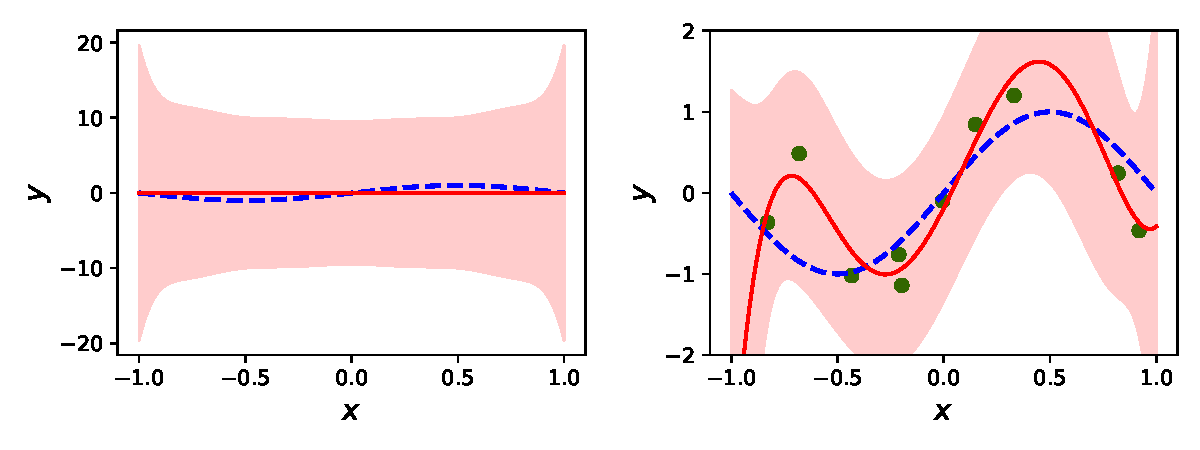
\includegraphics[width=0.9\textwidth]{../figures/bayesian_regression_1.pdf}
    \caption{10 data points}
  \end{subfigure}

  \begin{subfigure}{\textwidth}
    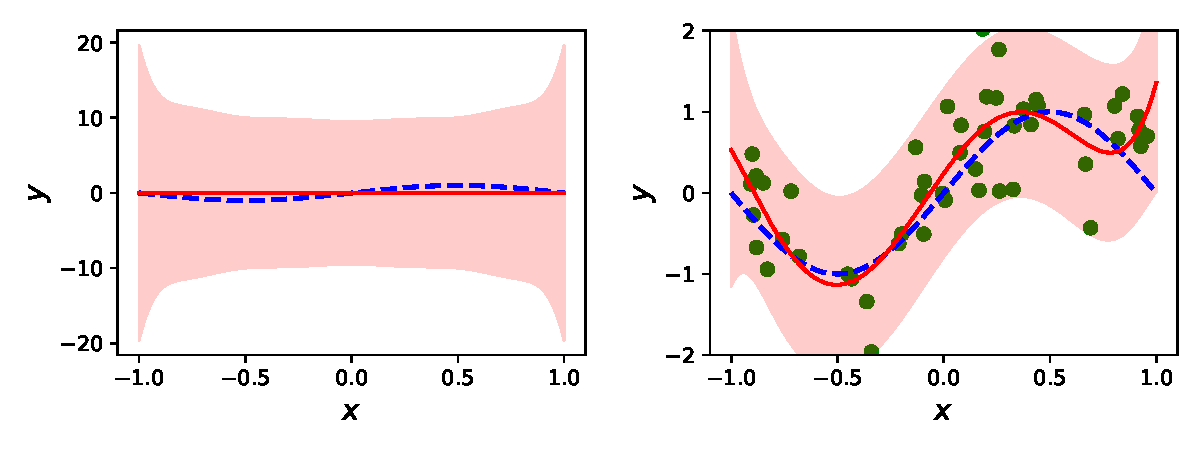
\includegraphics[width=0.9\textwidth]{../figures/bayesian_regression_2.pdf}
    \caption{50 data points}
  \end{subfigure}

  \begin{subfigure}{\textwidth}
    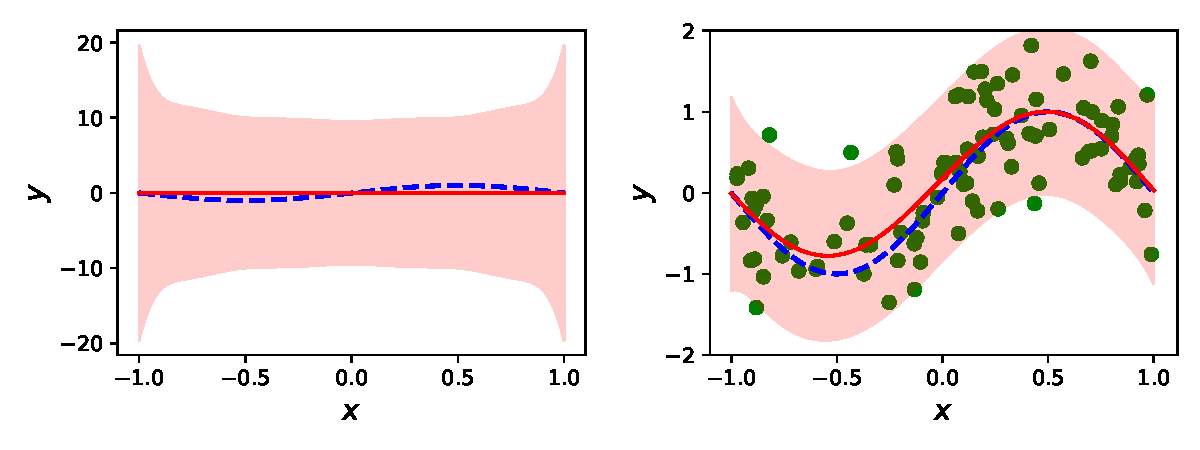
\includegraphics[width=0.9\textwidth]{../figures/bayesian_regression_3.pdf}
    \caption{100 data points}
  \end{subfigure}

  \caption{Bayesian regression with a degree 5 polynomial approximation,
  $\Vec{\theta} \sim \NormalDist(\Vec{0}, \Vec{16} \Mat{I}_6)$ prior and $\eta
  \sim \NormalDist(0, 0.25)$ noise model using different number of data points.
  The blue dashed lines represent true values, the green dots represent
  measurements, the red solid line is the mean of induced distribution on
  function values, the shaded red region is the $2\sigma$-uncertainty region of
  the same. The left panes correspond to the prior, and the right panes to the
  posterior. We observe that as the number of data points is increased, the
  posterior mean gradually approaches the true function---indicating the
  generalization error is decreasing.}
  \label{fig:regression}
\end{figure}

\subsubsection{Posterior Distribution}

From Bayes rule, we have
\begin{equation}
  \begin{split}
    -\log p(\Vec{\theta} \mid \Vec{x}, \Vec{y})
    &= -\log p(\Vec{\theta}) - \log p(\Vec{x}, \Vec{y} \mid \Vec{\theta}) +
    \text{const.} \\
    &= \frac{1}{2} (\Vec{\theta} - \Vec{\mu}_0)^\top \Mat{\Sigma}_0^{-1}
    (\Vec{\theta} - \Vec{\mu}_0) + \frac{1}{2 \sigma_\eta^2} \Norm{\Vec{y} -
    \Mat{\Phi}(\Vec{x})^\top \Vec{\theta}}^2 + \text{const.} \\
    &= \frac{1}{2} \Vec{\theta}^\top \left[\Mat{\Sigma}_0^{-1} +
    \frac{1}{\sigma_\eta^2} \Mat{\Phi}(\Vec{x}) \Mat{\Phi}(\Vec{x})^\top\right]
    \Vec{\theta} - \left[\Mat{\Sigma}_0^{-1} \Vec{\mu}_0 +
    \frac{1}{\sigma_\eta^2} \Mat{\Phi}(\Vec{x}) \Vec{y}\right]^\top \Vec{\theta}
    + \text{const.}
  \end{split}
\end{equation}
Clearly, we have
\begin{equation}
  \Vec{\theta} \mid \Vec{x}, \Vec{y} \sim \NormalDist(\Vec{\mu}, \Mat{\Sigma}),
  \quad
  \Mat{\Sigma}^{-1} = \Mat{\Sigma}_0^{-1} + \frac{1}{\sigma_\eta^2}
  \Mat{\Phi}(\Vec{x}) \Mat{\Phi}(\Vec{x})^\top,
  \quad
  \Vec{\mu} = \Mat{\Sigma} \left[\Mat{\Sigma}_0^{-1} \Vec{\mu}_0 +
  \frac{1}{\sigma_\eta^2} \Mat{\Phi}(\Vec{x}) \Vec{y}\right]
\end{equation}
and this allows us to predict the distribution of $y = \Vec{\phi}(x)^\top
\Vec{\theta} + \eta$ for any $x \in [-1, 1]$ as
\begin{equation}
  y \mid x, \Vec{x}, \Vec{y} \sim \NormalDist(\mu(x), \sigma(x)^2), \quad \mu(x)
  = \Vec{\phi}(x)^\top \Vec{\mu}, \quad \sigma(x)^2 = \Vec{\phi}(x)^\top
  \Mat{\Sigma} \Vec{\phi}(x) + \sigma_\eta^2
\end{equation}

\subsubsection{Numerical Results}

We apply this machinery to learn the function $f(x) = \sin(\pi x)$ on $[-1, 1]$.
We generate data points $(x_i, y_i)$ by first sampling $x_i$ uniformly in $[-1,
1]$, then computing $y_i = \sin(\pi x_i) + \eta_i$ with $\eta_i \sim
\NormalDist(0, 0.25)$. We assume a 5th degree polynomial expansion, and impose a
prior distribution of $\Vec{\theta} \sim \NormalDist(\Vec{0}, \sigma_\theta^2
\Mat{I}_6)$ with $\sigma_\theta = 4.0$.  In Figure~\ref{fig:regression}, we plot
the distribution of function values from the imposed prior on the parameters, as
well as the posterior after Bayesian inference.

\subsection{PAC-Bayesian Theory of Linear Regression}

While it is clear from Figure~\ref{fig:regression} that generalization error
tends to decrease as we increase the number of data points, Bayesian inference
does not provide any quantitative guarantee of this fact. This issue, however,
can be addressed in the context of PAC-Bayes learning.

We note that the likelihood term
\begin{equation}
  p(\Vec{x}, \Vec{y} \mid \Vec{\theta}) = C \exp(- \frac{1}{2 \sigma_\eta^2}
  \Norm{\Vec{y} - \Mat{\Phi}(\Vec{x})^\top \Vec{\theta}}^2)
\end{equation}
can be recovered as empirical risk $\hat{R}_S^L(\bm{\theta})$ with the loss
function
\begin{equation}
  L(\bm{\theta}, x, y) = \frac{1}{2 \sigma_\eta^2} (y - \Vec{\phi}(x)^\top
  \Vec{\theta})^2
\end{equation}
We will now show that this loss function is sub-gamma. Let us assume that the
true parameter value is $\Vec{\theta}^*$, then
\begin{equation}
  \begin{split}
    \Ev[\Vec{\theta}, x', y']{\exp(t [R_\CD^L(\Vec{\theta}) - L(\Vec{\theta},
    x', y')])}
    &= \Ev[\Vec{\theta}, x', y']{\exp(t \qty[\Ev[x, y]{L(\Vec{\theta}, x, y)} -
    L(\Vec{\theta}, x', y')])} \\
    &\leq \Ev[\Vec{\theta}]{\exp(t \Ev[x, y]{L(\Vec{\theta}, x, y)})} \\
    &= \Ev[\Vec{\theta}]{\exp(\frac{t}{2 \sigma_\eta^2} \Ev[x]{\Ev[y \mid x]{(y
    - \Vec{\phi}(x)^\top \Vec{\theta})^2}})} \\
    &= \Ev[\Vec{\theta}]{\exp(\frac{t}{2 \sigma_\eta^2}
    \qty(\Ev[x]{[\Vec{\phi}(x)^\top (\Vec{\theta} - \Vec{\theta}^*)]^2} +
    \sigma_\eta^2))} \\
    &= \Ev[\Vec{\theta}]{\exp(\frac{t}{2 \sigma_\eta^2} (\Vec{\theta} -
    \Vec{\theta}^*)^\top \Ev[x]{\Vec{\phi}(x) \Vec{\phi}(x)^\top} (\Vec{\theta}
    - \Vec{\theta}^*) + \frac{t}{2})} \\
    &\leq \Ev[\Vec{\theta}]{\exp(\frac{t}{2 \sigma_\eta^2} \kappa_{\phi, m}
    \Norm{\Vec{\theta} - \Vec{\theta}^*}^2 + \frac{t}{2})}
  \end{split}
\end{equation}
where we denote
\begin{equation}
  \kappa_{\phi, m} = \Norm{\Ev[x]{\Vec{\phi}(x) \Vec{\phi}(x)^\top}}_2
\end{equation}
We can evaluate this latest expectation with direct integration:
\begin{equation}
  \begin{split}
    \ln \Ev[\Vec{\theta}, x', y']{\exp(t [R_\CD^L(\Vec{\theta}) -
    L(\Vec{\theta}, x', y')])}
    &\leq \ln \Ev[\Vec{\theta}]{\exp(\frac{t}{2 \sigma_\eta^2} \kappa_{\phi, m}
    \Norm{\Vec{\theta} - \Vec{\theta}^*}^2 + \frac{t}{2})} \\
    &= -\frac{m}{2} \ln(1 - \frac{t \kappa_{\phi,m}
    \sigma_\theta^2}{\sigma_\eta^2}) + \frac{t \kappa_{\phi, m}}{2 \sigma_\eta^2
    - 2 t \kappa_{\phi, m} \sigma_\theta^2} \Norm{\Vec{\theta}^*}^2 +
    \frac{t}{2} \\
    &= - \frac{m}{2} \ln(1 - t c) + \frac{t c}{2 \sigma_\theta^2 (1 - t c)}
    \Norm{\Vec{\theta}^*}^2 + \frac{t}{2}
  \end{split}
\end{equation}
where $c = \kappa_{\phi, m} \sigma_\theta^2 / \sigma_\eta^2$. Now using
\begin{equation}
  - \ln(1 - x) \leq \frac{x (2 - x)}{2 (1 - x)} \quad \text{for all} \quad x \in
  [0, 1)
\end{equation}
we obtain
\begin{equation}
  \begin{split}
    \ln \Ev[\Vec{\theta}, x', y']{\exp(t [R_\CD^L(\Vec{\theta}) -
    L(\Vec{\theta}, x', y')])}
    &\leq \frac{m}{2} \frac{t c (2 - t c)}{2 (1 - t c)} + \frac{t c}{2
    \sigma_\theta^2 (1 - t c)} \Norm{\Vec{\theta}^*}^2 + \frac{t}{2} \\
    &= \frac{1}{2 (1 - t c)} \frac{m t c (2 - t c) \sigma_\theta^2 + 2 t c
    \Norm{\Vec{\theta}^*}^2 + 2 t \sigma_\theta^2 (1 - t c)}{2 \sigma_\theta^2}
    \\
    &= \frac{t^2 s^2}{2 (1 - t c)}
  \end{split}
\end{equation}
with
\begin{equation}
  s^2 = \frac{1}{t} \frac{[m c (2 - t c) + 2 (1 - t c)] \sigma_\theta^2 + 2 c
  \Norm{\Vec{\theta}^*}^2}{2 \sigma_\theta^2}
\end{equation}
Let us choose $c < 1$, then the value of $t = 1$ is acceptable, which
corresponds to $\lambda = n$. Now from Corollary~\ref{cor:alquier-sub-gamma} we
obtain
\begin{equation}
  \Ev[h \sim \rho]{R_\CD^L(h)} \leq \Ev[h \sim \rho]{\hat{R}_S^L(h)} +
  \frac{1}{n}\left[\KL{\rho}{\pi} + \ln \frac{1}{\delta}\right] +
  \frac{1}{2 (1 - c)} s^2
\end{equation}
with
\begin{equation}
  c = \frac{\kappa_{\phi, m} \sigma_\theta^2}{\sigma_\eta^2}, \quad s^2 =
  \frac{m c (2 - c) + 2 (1 - c)}{2} + \frac{c}{\sigma_\theta^2}
  \Norm{\Vec{\theta}^*}^2
\end{equation}

We now turn to estimating $\kappa_{\phi, m}$ for a specific choice of basis
functions and distribution on $x$. Let us denote
\begin{equation}
  \Mat{K} = \Ev[x]{\Vec{\phi}(x) \Vec{\phi}(x)^\top}
\end{equation}
Let us use the Legendre basis functions and uniform distribution on $[-1, 1]$;
then we have
\begin{equation}
  K_{ij} = \frac{1}{2} \int_{-1}^1 x P_{i - 1}(x) P_{j - 1}(x) \dd{x}
\end{equation}
For $i = 1$ we get $P_{i - 1}(x) = 1$, hence
\begin{equation}
  K_{1j} = \frac{1}{2} \int_{-1}^1 x P_{j - 1}(x) \dd{x} = \frac{1}{2}
  \int_{-1}^1 P_1(x) P_{j - 1}(x) \dd{x} = \frac{1}{3} \delta_{j, 2}
\end{equation}
For $i > 1$, we have
\begin{equation}
  x P_{i - 1}(x) = \frac{1}{2 i - 1} \qty[i P_i(x) + (i - 1) P_{i - 2}(x)]
\end{equation}
and therefore
\begin{equation}
  K_{ij} = \frac{i}{(2 i - 1) (2 i + 1)} \delta_{i, j - 1} + \frac{i - 1}{(2 i -
  3) (2 i - 1)} \delta_{i - 2, j - 1}
\end{equation}
It follows that $\Mat{K}$ is a symmetric tri-diagonal matrix with entries
\begin{equation}
  K_{ii} = 0, \quad K_{i + 1, i} = K_{i, i + 1} = \frac{i}{(2 i - 1) (2i + 1)}
\end{equation}
Now, for any matrix $\Mat{A}$ we have $\Norm{\Mat{A}}_2^2 \leq \Norm{\Mat{A}}_1
\Norm{\Mat{A}}_\infty$. Also for symmetric $\Mat{A}$ we have $\Norm{\Mat{A}}_1 =
\Norm{\Mat{A}}_\infty$. It follows that for our matrix $\Mat{K}$
\begin{equation}
  \kappa_{\phi, m} = \Norm{\Mat{K}}_2 \leq \Norm{\Mat{K}}_1 = \max_{1 \leq i
  \leq k} \sum_{j = 1}^m \Abs{K_{ij}} = \frac{7}{15}
\end{equation}
by direct evaluation.

With all this, we can now state the following:

\begin{proposition}[PAC-Bayes Bound for Bayesian Linear Regression]
  Let $\CD$ be a data distribution defined over $[-1, 1] \times \RR$ as follows:
  \begin{equation}
    \CD(x, y) = \UnifDist(x \mid -1, 1) \NormalDist(y \mid \Vec{\phi}(x)^\top
    \Vec{\theta}^*, \sigma_\eta^2)
  \end{equation}
  where $\Vec{\phi}(x) = (P_0(x), \ldots, P_{m - 1}(x))$ is constructed using
  Legendre polynomials. Let $\Vec{\theta} \sim \NormalDist(\Vec{0},
  \sigma_\theta^2 \Mat{I}_m)$ be a prior distribution on the parameter set
  $\RR^m$. Then given the square loss function
  \begin{equation}
    L(\Vec{\theta}, x, y) = \frac{1}{2 \sigma_\eta^2} (y - \Vec{\phi}(x)^\top
    \Vec{\theta})^2
  \end{equation}
  and real number $\delta \in (0, 1)$, the following holds with probability at
  least $1 - \delta$ over $S \sim \CD^n$ i.i.d.
  \begin{equation}
    \Ev[h \sim \hat{\rho}]{R_\CD^L(h)} \leq \Ev[h \sim
    \hat{\rho}]{\hat{R}_S^L(h)} + \frac{1}{n}\left[\KL{\hat{\rho}}{\pi} + \ln
    \frac{1}{\delta}\right] + \frac{1}{2 (1 - c)} s^2
  \end{equation}
  where $\hat{\rho}$ is the posterior obtained from Bayesian inference and
  \begin{equation}
    c = \frac{7 \sigma_\theta^2}{15 \sigma_\eta^2}, \quad s^2 = \frac{m c (2 -
    c) + 2 (1 - c)}{2} + \frac{c}{\sigma_\theta^2} \Norm{\Vec{\theta}^*}^2
  \end{equation}
\end{proposition}

Clearly, as the number of data points $n$ is increased, the difference between
generalization error and the empirical error decreases; however they don't
converge. The difference depends on four aspects: number of data points $m$,
prior standard deviation $\sigma_\theta$, noise standard deviation
$\sigma_\eta$ and the distance of the true parameter values $\Vec{\theta}^*$
from the origin. Additionally
\begin{itemize}
  \item
    To satisfy the necessary $c < 1$ constraint, we need to balance the prior
    variance and noise variance. As the noise variance is increased, we also
    need to increase the prior variance.
  \item
    As the number of data points is increased, the distance between the
    generalization and empirical errors also increase linearly.
  \item
    As the true parameter value $\Vec{\theta}^*$ moves away from the origin, the
    gap also increases quadratically with the distance. This can be
    counterbalanced by increasing the prior variance, which requires us to
    increase the noise variance.
\end{itemize}


\bibliography{references}
\bibliographystyle{plainnat}

\end{document}
